\chapter{Design}
Stratergy?


\section{Overall Architecture}


\section{Data Structures}

\section{Class Diagram}
hello
\begin{figure}[H]
  \centering
   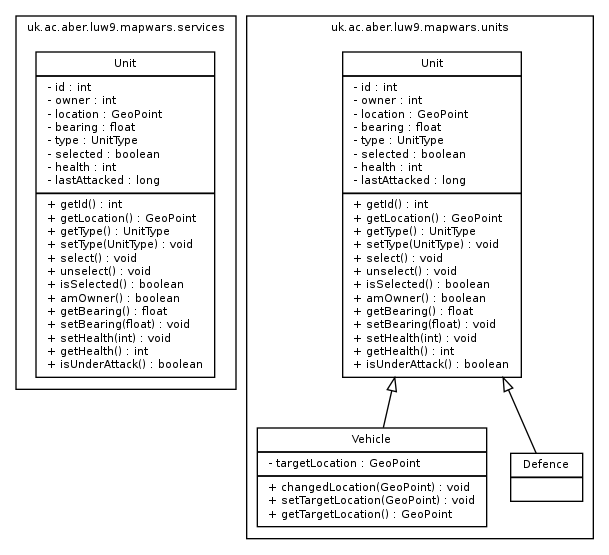
\includegraphics[width=1\textwidth]{Images/diagrams/client-class.png}
  \caption{Client class diagram}
  \label{fig:client}
\end{figure}

\section{Use Case Diagram}





\subsection{Language}
Developing applications for the Android OS restricts the language choice to just Java combined with an Android framework. This results in code written with Java syntax but are not entirely synonymous with Java. Code is converted from Java Virtual Machine (JVM) compatible code to code that can be run by Dalvik, the vitual machine used by Android. This conversion optimizes the code to be run on devices with limited memory and processing power.

For the server portion of the application it was important to choose a language that would aid in the rapid development methodology outlined for the project. Python is a general purpose high-level programming language that has a relatively small learning curve as well as some personnel background knowledge. It is designed with the express purpose of being highly readable by forcing well formatted code and using English keywords. 

As the chosen hardware for the server is limited in processing power and memory it is important keep overheads to a minimum, which Python does fairly well. If Java had been used a much more powerful server would have been needed to support the same number of processes due to the overheads introduced by the JVM. However there would have been a number of advantages to using the same language as the client. These include a greater understanding of the language as it is used more extensively but more importantly would be code reuse. The client and server both perform many of the same procedures and could have sped up development time and increased accuracy and interoperability as the same packages could have been utilized.

The server also required a persistent data store to keep an overview of the users and units between downtime or server migration. The requirements specified matched closely to those given when choosing Python as the programming language. 


    Non-proprietary
    Simple, zero-configuration database
    Relational makes things easy
    Lightweight
    Previous knowledge of SQL makes that a preferable language of choice
    Simple python implementation.

A nice looking option was KirbyBase (http://wiki.python.org/moin/KirbyBase) it matched all of the requirements and being purely python based was a plus. It is a flat-file database so was simple to configure and lightweight, it also had the flexibility of running both as part of an application or in a client-server configuration. Unfortunately development stopped in 2006 and the libraries website has since been taken offline.

MongoDB  

One long term problem that comes with SQLite is that it could not be run in a client-server configuration restricting the application to a single server. As the popularity and interest in the game increases so would the demand on the server meaning that a more complex, distributed server model would be needed. This is outside of the scope of the current project so this was deemed to be an acceptable compromise.

\section{User Interface}
When developing any application for a small form factor it is important to consider how the user interface can be minimized, and to not clutter the display making precise controls difficult. This is especially important when trying to fit all the functionality of a \gls{rts} game within the small form factor of a mobile device. To get around this problem only the essential controls will be included with only a portion of these being accessible from the main game screen.

\begin{figure}[H]
\centering
\begin{minipage}{.5\textwidth}
  \centering
  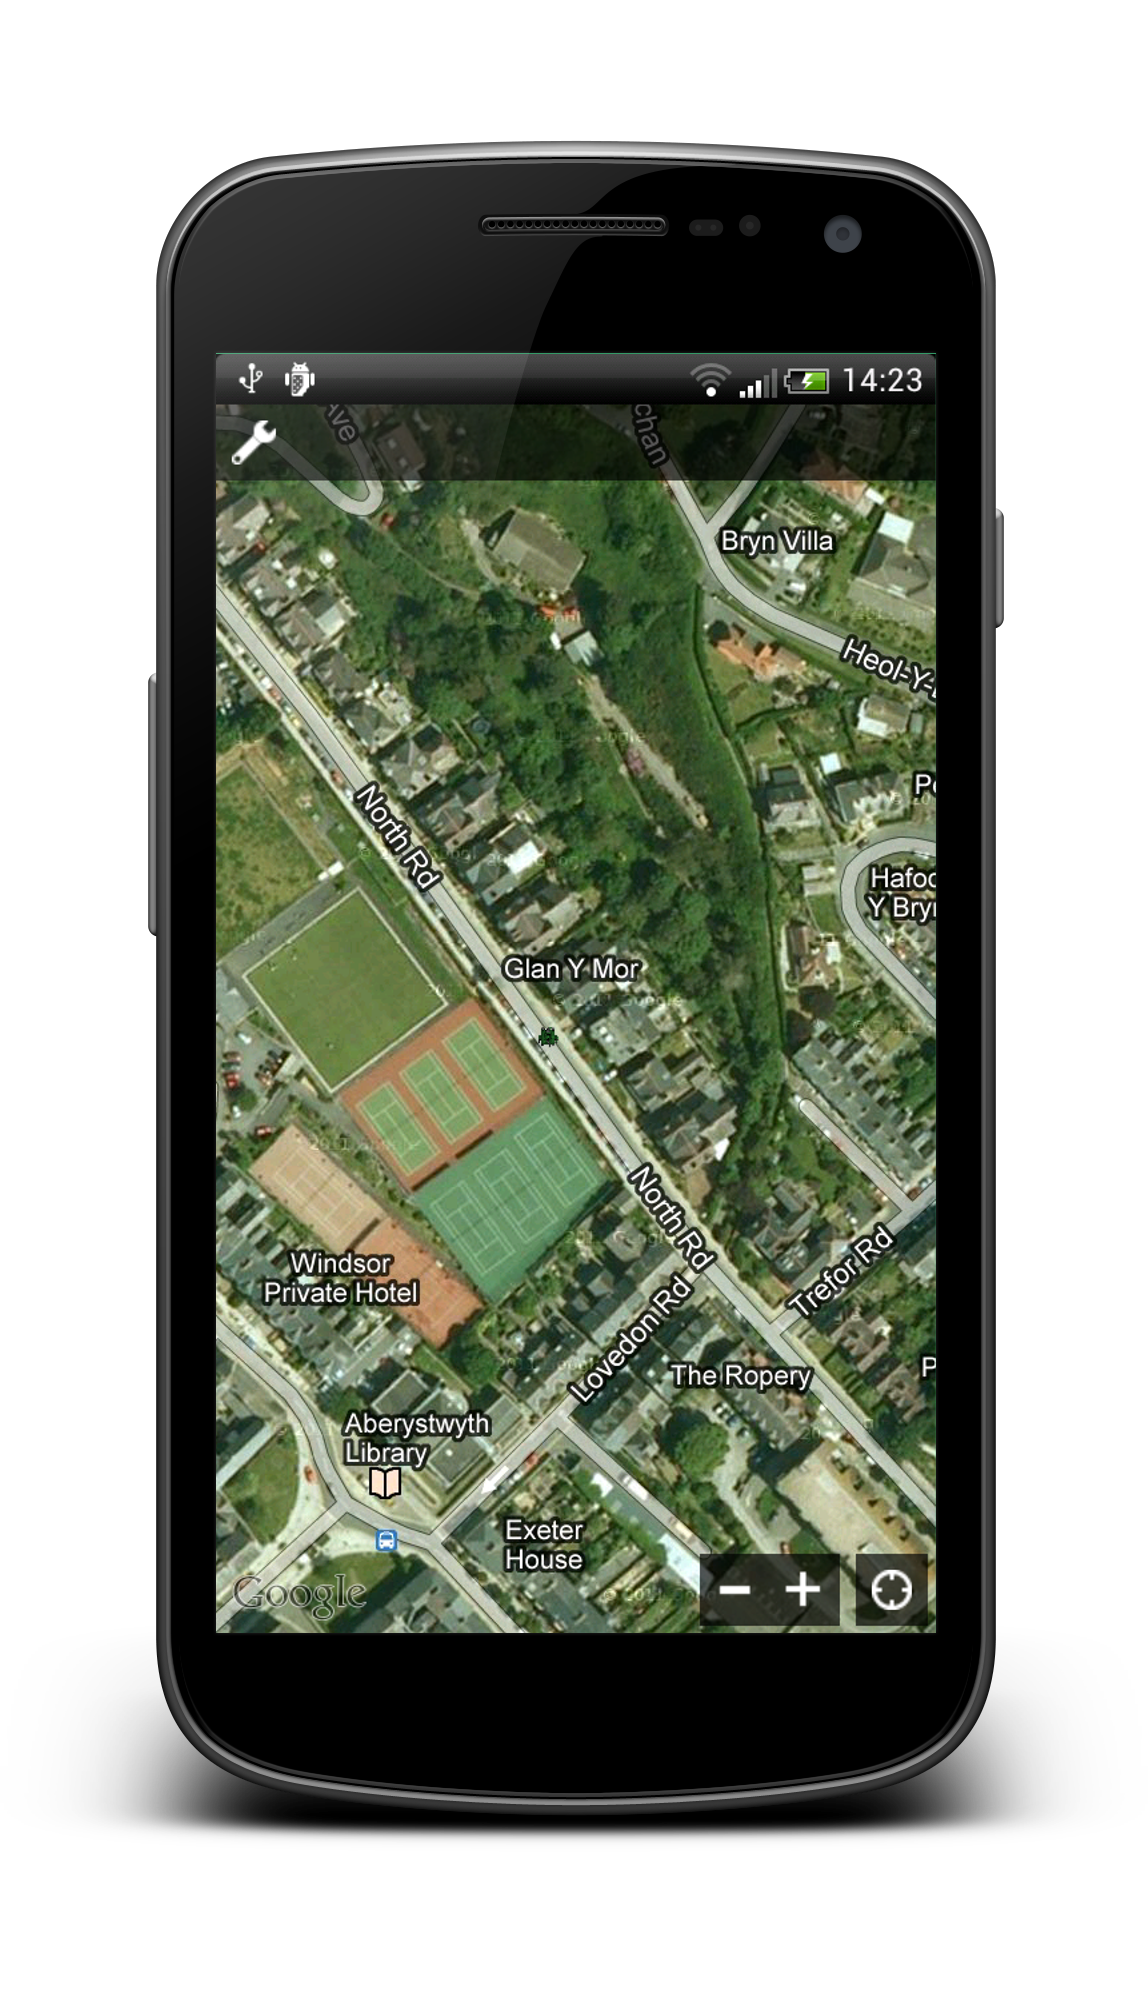
\includegraphics[width=.4\linewidth]{Images/maps-google.png}
  \captionof{figure}{Insert design of game map}
  \label{fig:test1}
\end{minipage}%
\begin{minipage}{.5\textwidth}
  \centering
  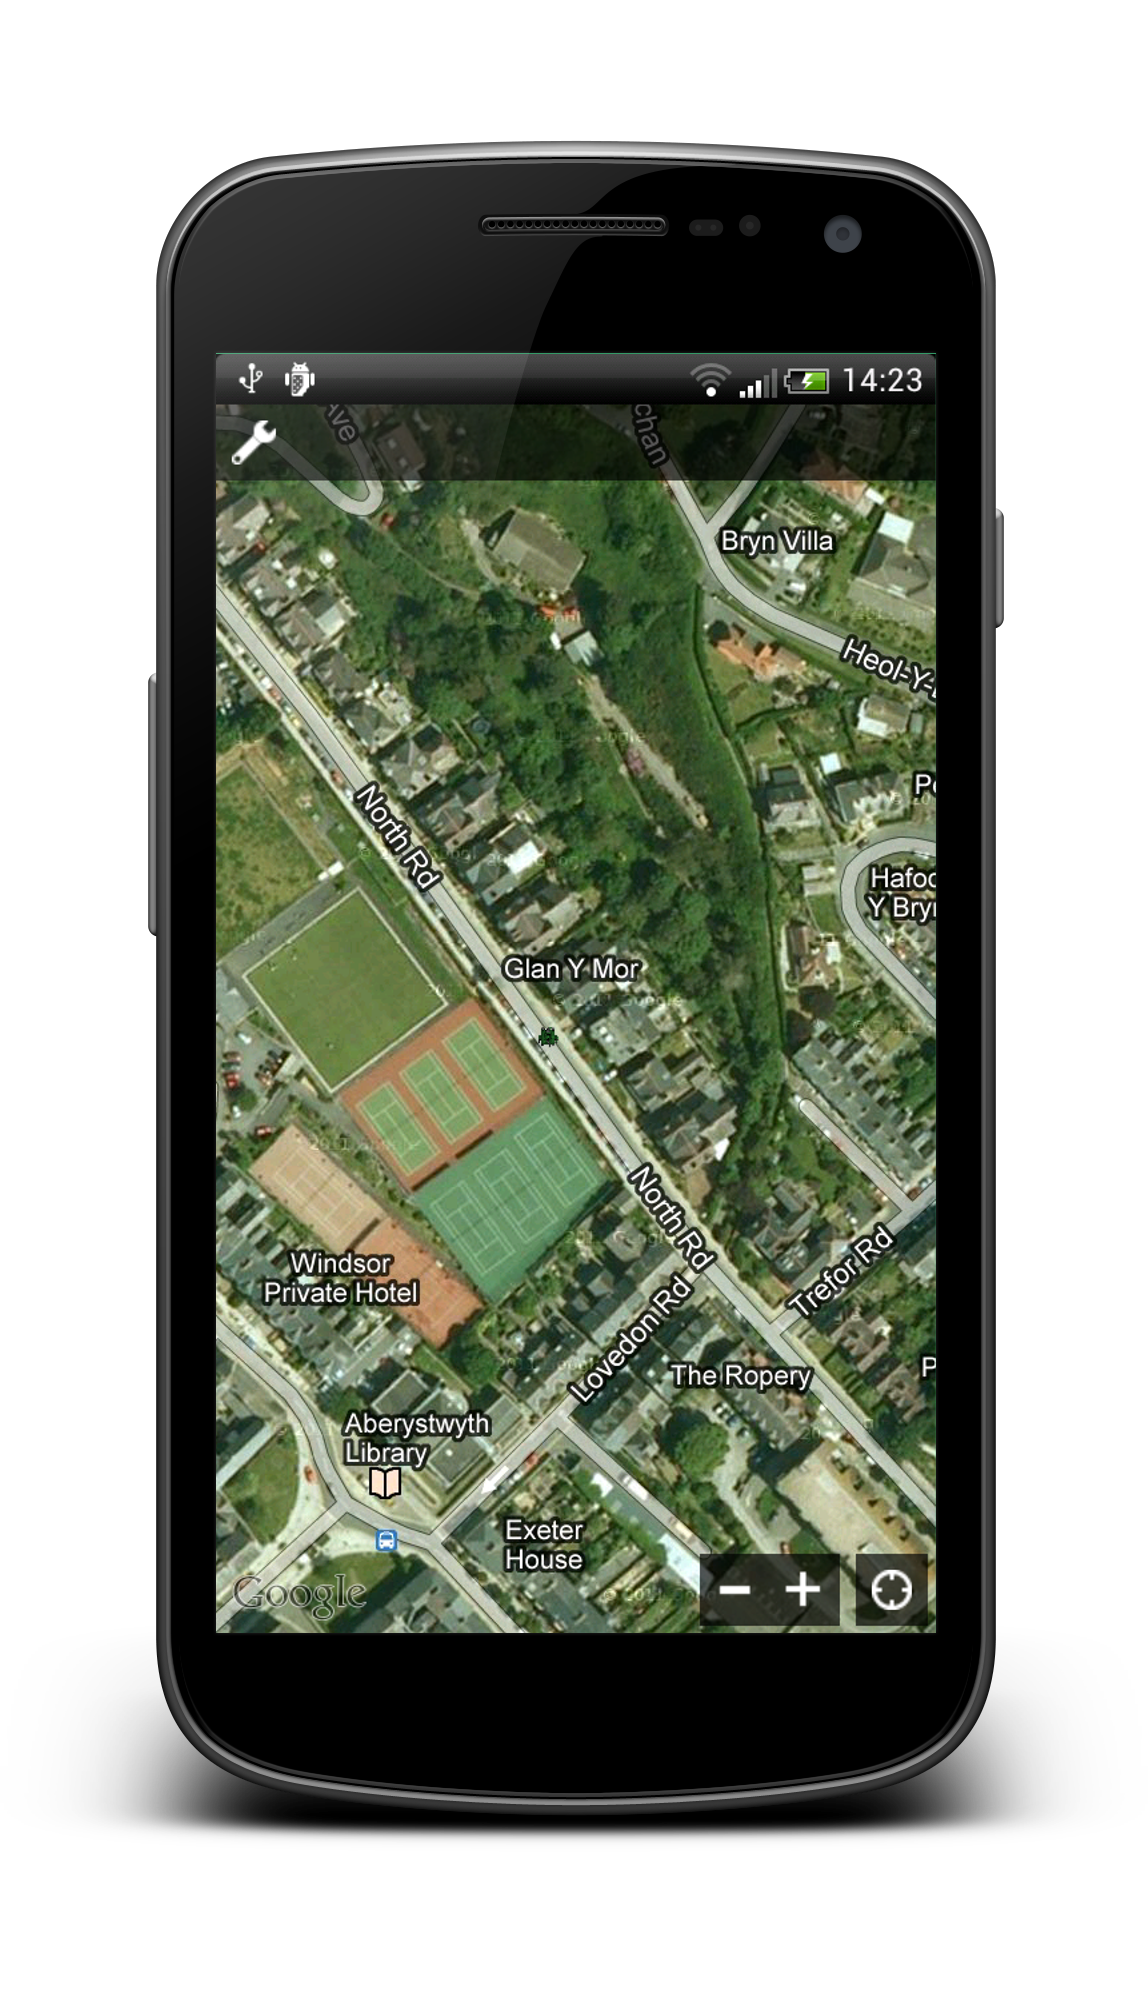
\includegraphics[width=.4\linewidth]{Images/maps-google.png}
  \captionof{figure}{Insert design of game map menu}
  \label{fig:test2}
\end{minipage}
\end{figure}

 Figure \ref{fig:test2}

